\chapter{Υλοποίηση της εφαρμογης}

%Το \en{Lorem Ipsum} είναι απλά ένα κείμενο χωρίς νόημα για τους επαγγελματίες της τυπογραφίας και στοιχειοθεσίας \cite{LoremIpsumAll}. Το \en{Lorem Ipsum} είναι το επαγγελματικό πρότυπο όσον αφορά το κείμενο χωρίς νόημα, από τον 15ο αιώνα, όταν ένας ανώνυμος τυπογράφος πήρε ένα δοκίμιο και ανακάτεψε τις λέξεις για να δημιουργήσει ένα δείγμα βιβλίου. Όχι μόνο επιβίωσε πέντε αιώνες, αλλά κυριάρχησε στην ηλεκτρονική στοιχειοθεσία, παραμένοντας με κάθε τρόπο αναλλοίωτο. Έγινε δημοφιλές τη δεκαετία του '60 με την έκδοση των δειγμάτων της \en{Letraset} όπου περιελάμβαναν αποσπάσματα του \en{Lorem Ipsum}, και πιο πρόσφατα με το λογισμικό ηλεκτρονικής σελιδοποίησης όπως το \en{Aldus PageMaker} που περιείχαν εκδοχές του \en{Lorem Ipsum}.
\section{Ανάπτυξη με το  \en{Django framework}}

\subsection{Δημιουργία \en{Models}}

Η διαδικτυακή πύλη χρησιμοποιεί μια βάση δεδομένων \en{SQLite}. Αυτή η βάση δεδομένων περιέχει τρία
μοντέλα τα οποία ορίζονται στο αρχείο \en{models.py}. Στην εικόνα 6.1 φαίνονται τα μοντέλα αυτά.

\FloatBarrier

\begin{figure}[htb]
	\centering
	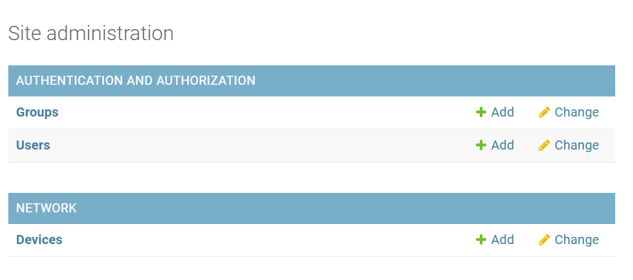
\includegraphics[width=0.9\textwidth]{graphics/models_2.png}
	\caption{Μοντέλα}
\end{figure}

\FloatBarrier


Η διαδικτυακή πύλη περιέχει την κλάση \en{Device}, η οποία δέχεται ως ορίσματα το όνομα, τη διεύθυνση \en{IP}, το όνομα χρήστη, τον κωδικό πρόσβασης, τον κρυφό κωδικό και το μοντέλο της συσκευής. Για κάθε μία από αυτές τις συσκευές που δημιουργούμε, καταγράφεται μια αντίστοιχη εγγραφή στη βάση δεδομένων. Το αντικείμενο που δημιουργείται δηλαδή η συσκευή προς δοκιμή περιλαμβάνει πεδία που αξιοποιούνται από τις συναρτήσεις του αρχείου \en{views.py}. Με αυτόν τον τρόπο, τα πεδία του αντικειμένου αποθηκεύονται και χρησιμοποιούνται ως ορίσματα μέσα στις συναρτήσεις, διευκολύνοντας τη διαχείριση και την επεξεργασία των δεδομένων της συσκευής




\subsection{\en{Views} και \en{Urls}}


 Τα αρχεία \en{Urls} καθορίζουν τη δρομολόγηση των \en{URL} της εφαρμογής. Οι διευθύνσεις \en{URL} που αντιστοιχούν στα μοτίβα που περιγράφονται στο αρχείο \en{urls.py} προωθούνται στην αντίστοιχη συνάρτηση στο αρχείο \en{views.py}. Η αντιστοίχιση πραγματοποιείται σειριακά από πάνω προς τα κάτω στο αρχείο \en{urls.py} όπως φαίνεται στη εικόνα 6.2. 

\FloatBarrier

\begin{figure}[htb]
	\centering
	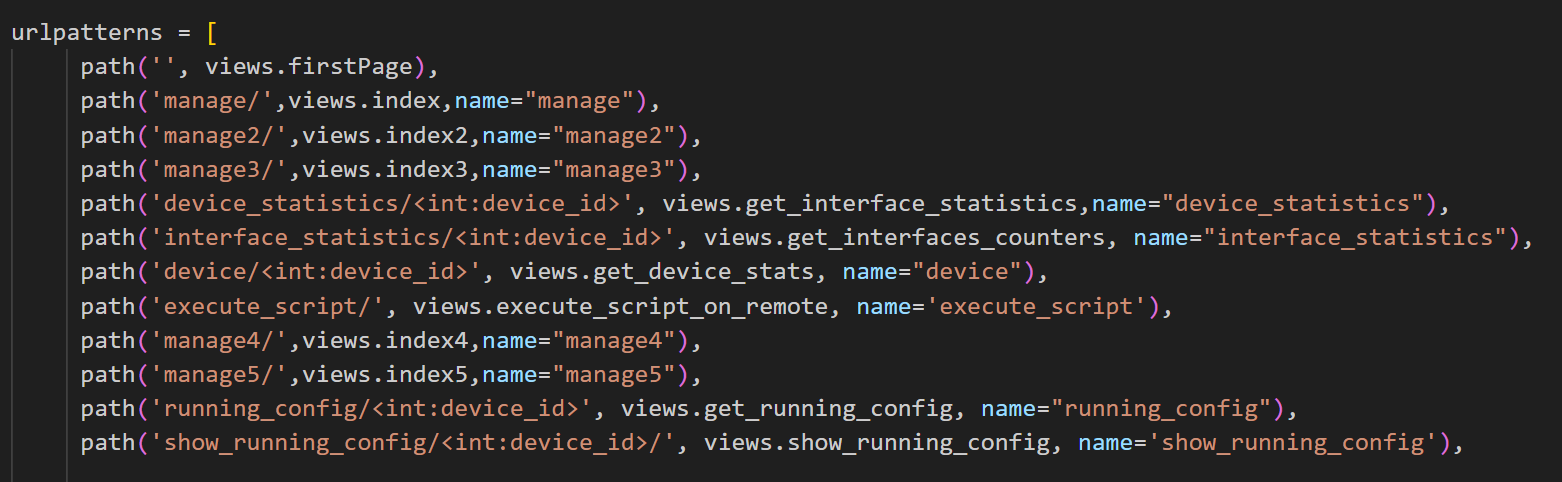
\includegraphics[width=0.9\textwidth]{graphics/urlpy.png}
	\caption{\en{url.py} }
\end{figure}

\FloatBarrier

Παρόλο που σε αυτό το έργο υλοποιήθηκε ακριβής αντιστοίχιση των \en{URL}, το \en{Django} παρέχει τη 
δυνατότητα χρήσης ταυτοποίησης μέσω κανονικών εκφράσεων. Στην εικόνα που ακολουθεί, παρουσιάζονται οι 
διευθύνσεις \en{URL} του \en{API}, όπου κάθε διεύθυνση αντιστοιχεί σε μια συνάρτηση στο αρχείο \en{api1/views.py}, 
η οποία καταλήγει στην εκτέλεση του αντίστοιχου σεναρίου



Οι συναρτήσεις σε ένα αρχείο \en{views.py} καλούνται όταν η δεδομένη διεύθυνση \en{URL} που αποστέλλεται από το
χρήστη ταιριάζει με το αντίστοιχο μοτίβο \en{URL} στο αρχείο \en{urls.py}. Παράμετροι που αποστέλλονται μέσω κλήσης
\en{HTTP} εισέρχονται στην αντίστοιχη συνάρτηση μέσω παραμέτρων ή σώματος αίτησης. Στο αρχείο \en{views.py} του \en{API}, η συνάρτηση εκτελεί το σενάριο
κώδικα με τις δεδομένες παραμέτρους εισόδου. Όταν τελειώσει η εκτέλεση του κώδικα δέσμης ενεργειών,
το αποτέλεσμα επιστρέφεται στη συνάρτηση \en{views} και μεταβιβάζεται ως πλαίσιο στο αντίστοιχο αρχείο \en{.html} για την εμφάνιση των αποτελεσμάτων στον χρήστη που εκτέλεσε το σενάριο.
Ένα παράδειγμα τριών διαφορετικών συνάρτησεων σε ένα αρχείο \en{views.py} μπορείτε να δείτε στο σχήμα 6.3.

\FloatBarrier

\begin{figure}[htb]
	\centering
	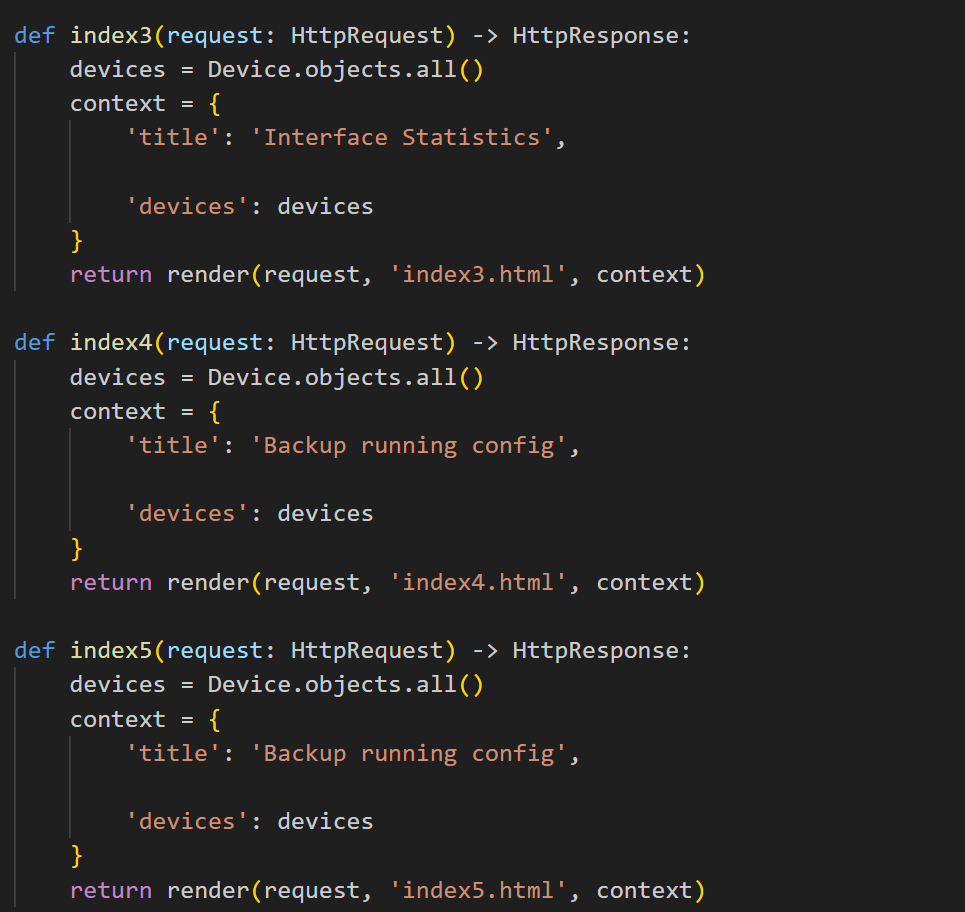
\includegraphics[width=0.9\textwidth]{graphics/viewspy.png}
	\caption{\en{views.py} }
\end{figure}

\FloatBarrier

\subsection{\en{User Interface (Templates)}}


Σε κάθε συνάρτηση του αρχείου \en{views.py}, το \en{Django} αποδίδει το αντίστοιχο πρότυπο \en{.html}
αρχείο με ένα συγκεκριμένο πλαίσιο. Η λογική είναι ότι κάθε \en{HTTP Request} που δέχεται όταν ο χρήστης επιδρά με την εφαρμογή απαντιέται με ένα αντίστοιχο \en{HTTP Response} . Τα δεδομένα στο πλαίσιο εμφανίζονται
στο \en{.html} μέσα από το \en{HTTP Response}, εάν το \en{.html} έχει παραμετροποιηθεί κατάλληλα. Ένα παράδειγμα \en{.html} με
τον συντακτικό κώδικα για τον τρόπο πρόσβασης στα δεδομένα του πλαισίου παρουσιάζεται στην εικόνα 6.4.

\FloatBarrier

\begin{figure}[htb]
	\centering
	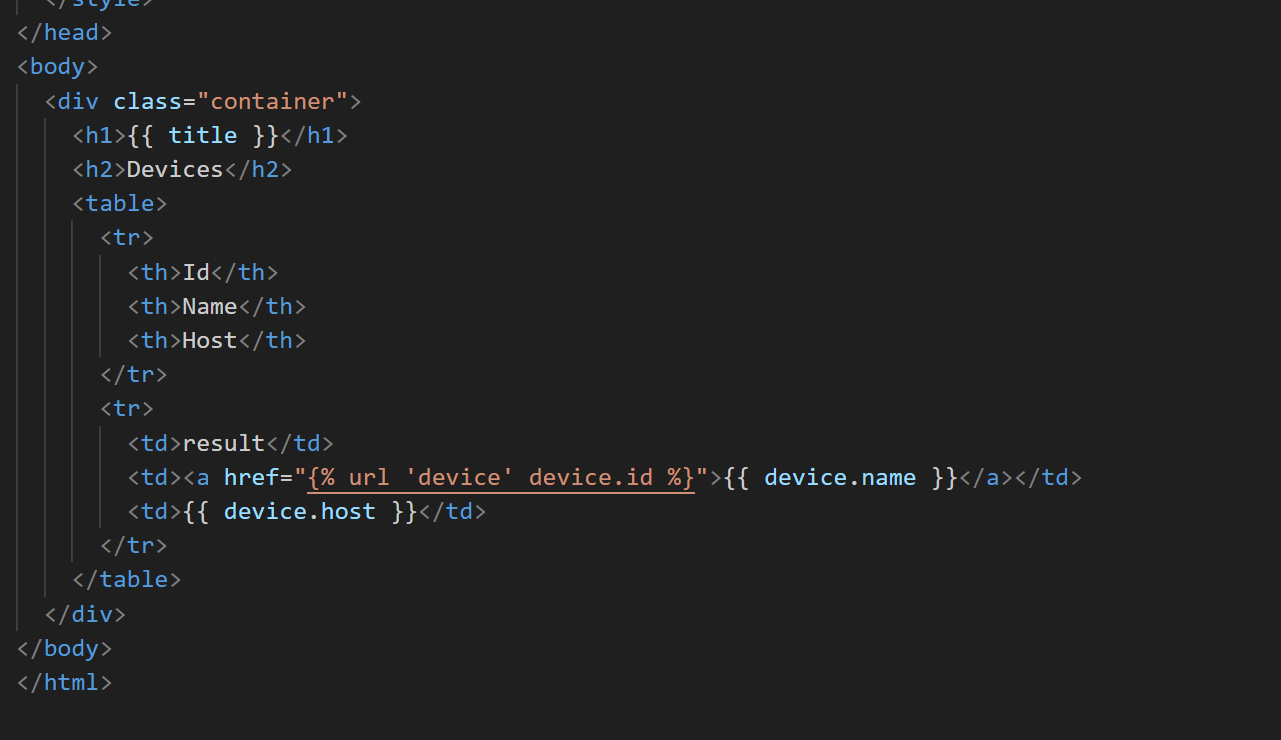
\includegraphics[width=0.9\textwidth]{graphics/html_template.png}
	\caption{Παράδειγμα \en{html} αρχείου }
\end{figure}

\FloatBarrier

Έτσι όλη η διαθέσιμη λειτουργικότητα που παρέχεται στον χρήστη της εφαρμογής διαχείρισης δικτύου υλοποιείται με την χρήση \en{URLs} (κλήσεις συναρτήσεων και \en{html} αρχείων). Έτσι για παράδειγμα για την λειτουργία \en{Statistics} : 

\begin{itemize}
    \item Ο χρήστης επισκέπτεται το \en{URL} \en{/manage3}. 
    \item Ο ορισμός του \en{URL} στο \en{urls.py} κατευθύνει το αίτημα στη συνάρτηση \en{index2} στο \en{views.py}.
    \item Με αυτό τον τρόπο ο χρήστης κάνει ένα \en{HTTP Request}. Η συνάρτηση \en{index2} συλλέγει τα δεδομένα (\en{context-data}) που χρειάζονται για την προβολή.
    \item Η συνάρτηση \en{index2} επιστρέφει τα δεδομένα στη σελίδα \en{index2.html} επιστρέφοντας το μέσα από ένα \en{HTTP Response}.
    \item Το \en{template} \en{index2.html} λαμβάνει τα δεδομένα και τα εμφανίζει στον χρήστη.
\end{itemize}


\section{\en{REST API Integration} και διασύνδεση με το \en{SSH protocol}}

 Το \en{REST API Integration} διαδραματίζει κρίσιμο ρόλο στη 
διπλωματική εργασία, καθώς επιτρέπει την αλληλεπίδραση μεταξύ των 
διαφόρων συστημάτων και την ανταλλαγή δεδομένων μέσω του διαδικτύου. 
Το \en{REST} (\en{Representational State Transfer}) είναι μια 
αρχιτεκτονική προσέγγιση που χρησιμοποιεί τα πρωτόκολλα \en{HTTP} 
για την εκτέλεση λειτουργιών όπως η ανάκτηση, η δημιουργία, η 
ενημέρωση και η διαγραφή δεδομένων. Με την υλοποίηση \en{REST APIs}, 
καθίσταται δυνατή η διαλειτουργικότητα της εφαρμογής με άλλες 
υπηρεσίες, διευκολύνοντας τη σύνθεση πολύπλοκων λειτουργιών από 
διάφορες πηγές. Στο πλαίσιο της διπλωματικής, το \en{REST API} 
χρησιμοποιείται για την διαχείριση δικτυακών συσκευών, παρακολούθηση 
στατιστικών, εκτέλεση εντολών, διασφαλίζοντας την ασφάλεια και την 
αποδοτικότητα της επικοινωνίας μέσω διαφανών και επεκτάσιμων 
τεχνολογιών. Το \en{REST} δεν χρησιμοποιείται για την επικοινωνία της εφαρμογής
και των συσκευών αλλα εσωτερικά ως μηχανισμός δρομολόγησης προκειμένου η εφαρμογή
να μπορεί να φέρει στον χρήστη το σωστό αποτέλεσμα. Η διαχείρηση των δικτυακών
συσκευών γίνεται με το πρωτόκολλο \en{SSH}.

Προσπαθώντας μέσα από το \en{wireshark} να πιάσουμε την κίνηση μεταξύ
\en{WSL} και δικτυακής συσκευής κάναμε το παρακάτω πείραμα προκειμένου να κατανοήσουμε 
πως επικοινωνεί η εφαρμογή με τις συσκευές. Πατάμε το κουμπί \en{R1 Testing} όπως φαίνεται στο σχήμα 6.5. και στο \en{Wireshark} κάνουμε \en{capture}
το \en{interface eth0} του \en{WSL} προκειμένου να δούμε τι γίνεται όταν εμείς πατάμε
το κουμπί για μια λειτουργία. Τα κουμπιά έχουν σχεδιαστεί έτσι ώστε, με το πάτημά τους, να σε κατευθύνουν μέσω συνδέσμου (\en{link}) στη λειτουργία που επιθυμείς να εκτελέσεις.


\FloatBarrier

\begin{figure}[htb]
	\centering
	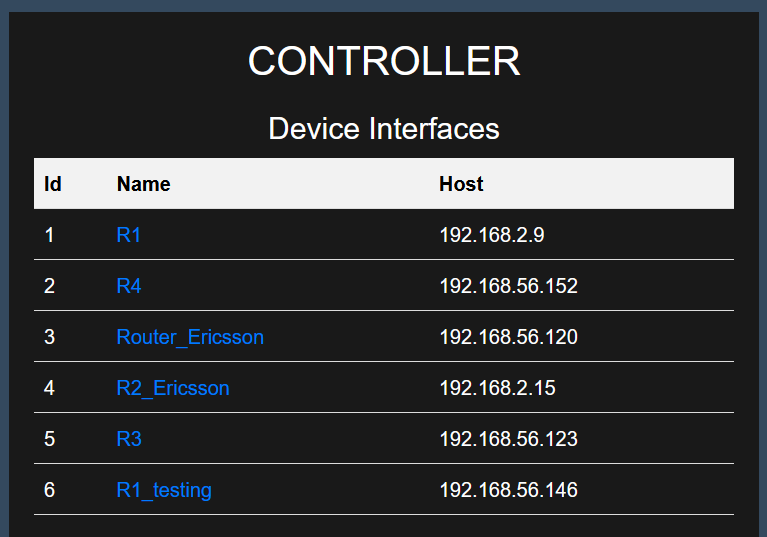
\includegraphics[width=0.9\textwidth]{graphics/r1_testing.png}
	\caption{Παράδειγμα \en{wireshark} }
\end{figure}

\FloatBarrier




\begin{figure}[htb]
	\centering
	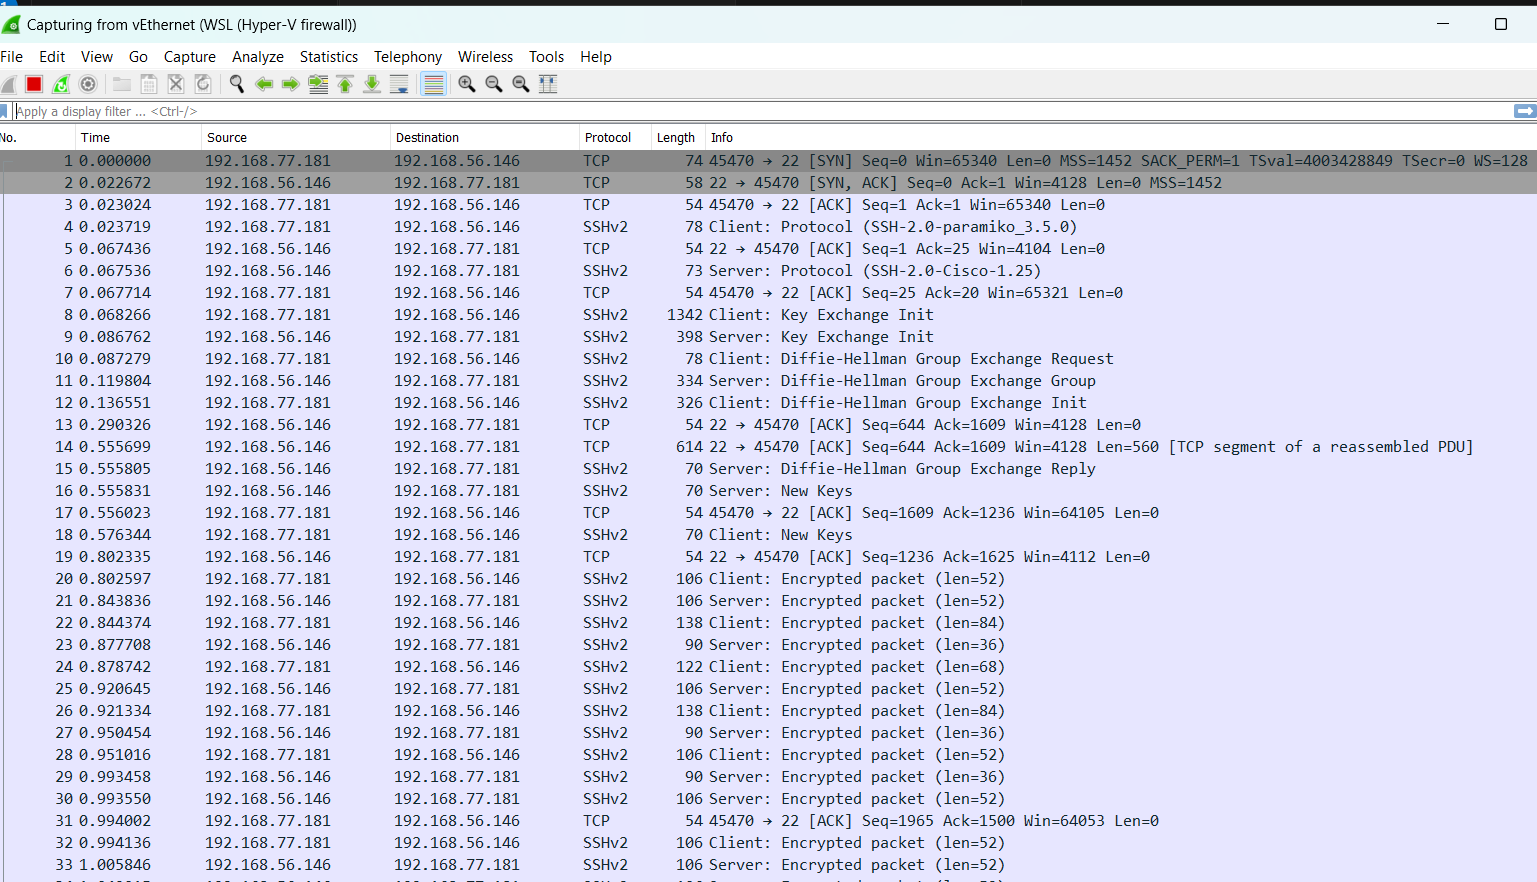
\includegraphics[width=0.9\textwidth]{graphics/wireshark.png}
	\caption{Παράδειγμα \en{wireshark} }
\end{figure}

\FloatBarrier

Αυτή η ακολουθία του σχήματος 6.6 αντιπροσωπεύει μια τυπική, ασφαλή σύνδεση \en{SSH}. Στο αρχείο \en{pcap} που καταγράψαμε, αποτυπώνεται η διαδικασία εγκαθίδρυσης μιας σύνδεσης \en{TCP} (\en{SYN, SYN/ACK, ACK}). Συγκεκριμένα, στο πρώτο πακέτο παρατηρούμε το \en{SYN}, το οποίο αποστέλλεται   προς τη συσκευή. Στη συνέχεια, η συσκευή αποκρίνεται με \en{SYN/ACK}, επιβεβαιώνοντας την επικοινωνία. Τέλος, στο τρίτο πακέτο, απαντάμε με \en{ACK}, ολοκληρώνοντας έτσι τη διαδικασία σύναψης της σύνδεσης.

Μετά ακολουθεί η διαπραγμάτευση πρωτοκόλλου \en{SSH} και στο τέλος η έναρξη της κρυπτογραφημένης επικοινωνίας την οποία δε μπορούμε να δούμε. Όμως μπορούμε να δούμε τι επιστρέφεται 
απο το \en{cli} του \en{Django server} στην  εικόνα 6.7.

\FloatBarrier
\begin{figure}[htb]
	\centering
	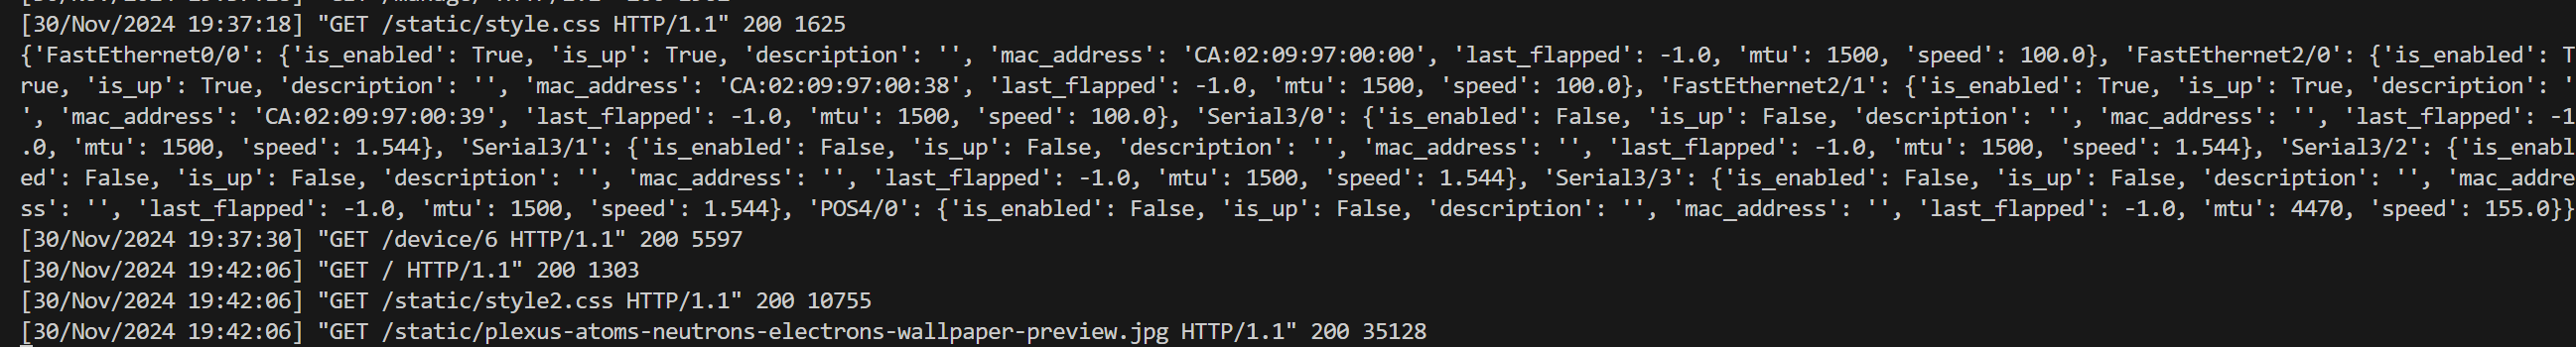
\includegraphics[width=0.9\textwidth]{graphics/rest.png}
	\caption{Απάντηση συσκευής}
\end{figure}

\FloatBarrier




%\begin{equation}
%	y = \alpha x + \beta
%\end{equation}

%Αντίθετα με αυτό που θεωρεί η πλειοψηφία, το \en{Lorem Ipsum} δεν είναι απλά ένα τυχαίο κείμενο. Οι ρίζες του βρίσκονται σε ένα κείμενο Λατινικής λογοτεχνίας του 45 π.Χ., φτάνοντας την ηλικία του πάνω από 2000 έτη.


%\begin{figure}[htb]
%	\centering
%	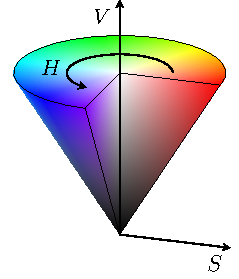
\includegraphics{tikz/hsv_cone/hsv_cone.pdf}
%	\caption{Ο χρωματικός χώρος \en{HSV}.}
%\end{figure}
